% =====================================================================
% Gamson's Law or a Formateur Premium? -- full paper
% Build: latexmk -pdf main.tex   (numbers come from ../report/numbers.tex and
% tab_*.tex, both generated from results/ by scripts/make_figures.py and
% scripts/paper_tables.py)
% =====================================================================
\documentclass[11pt,a4paper]{article}
\usepackage[T1]{fontenc}
\usepackage[utf8]{inputenc}
\usepackage{mathtools,amssymb,amsthm}
\usepackage{lmodern,microtype}
\usepackage[a4paper,margin=25mm]{geometry}
\usepackage{graphicx,booktabs,xcolor,enumitem}
\usepackage[font=small,labelfont=bf]{caption}
\usepackage[round,authoryear]{natbib}
\usepackage[colorlinks=true,linkcolor=blue!50!black,citecolor=blue!50!black,urlcolor=blue!50!black]{hyperref}
\usepackage[nameinlink,capitalise,noabbrev]{cleveref}
\captionsetup[table]{position=top,skip=4pt}
\setlist{itemsep=1pt,topsep=3pt}

\newtheorem{proposition}{Proposition}
\newtheorem{definition}{Definition}
\newtheorem{remark}{Remark}
\crefname{proposition}{Proposition}{Propositions}

\newcommand{\repo}{https://github.com/bot2048/cabinet-bargaining-marl}
\newcommand{\code}[1]{\href{\repo/blob/main/#1}{\texttt{\small #1}}}
\newcommand{\E}{\mathbb{E}}
\newcommand{\BF}{\mathrm{BF}}
% generated by scripts/make_figures.py -- do not edit
\newcommand{\AfDemFormHi}{0.51}
\newcommand{\AfDemFormLo}{0.44}
\newcommand{\AfDemMaxDev}{0.02}
\newcommand{\AfDemSeeds}{3}
\newcommand{\AfDemSlope}{\ensuremath{-}0.02 to +0.12}
\newcommand{\AfPropFormHi}{0.73}
\newcommand{\AfPropFormLo}{0.65}
\newcommand{\AfPropMaxDev}{0.23}
\newcommand{\AfPropSeeds}{3}
\newcommand{\AfPropSlope}{+0.38 to +0.75}
\newcommand{\AtDemDummy}{0.0\%}
\newcommand{\AtDemFormHi}{0.47}
\newcommand{\AtDemFormLo}{0.39}
\newcommand{\AtDemMaxDev}{0.03}
\newcommand{\AtDemSeeds}{3}
\newcommand{\AtDemSlope}{+0.06 to +0.28}
\newcommand{\AtPropBigHi}{0.71}
\newcommand{\AtPropBigLo}{0.65}
\newcommand{\AtPropDumHi}{0.39}
\newcommand{\AtPropDumLo}{0.36}
\newcommand{\AtPropDummy}{5.4\%}
\newcommand{\AtPropFormHi}{0.71}
\newcommand{\AtPropFormLo}{0.36}
\newcommand{\AtPropMaxDev}{0.20}
\newcommand{\AtPropSeeds}{3}
\newcommand{\AtPropSlope}{\ensuremath{-}0.12 to +1.63}
\newcommand{\BaseBeta}{+0.468}
\newcommand{\BaseCollapse}{+0.000}
\newcommand{\BaseDg}{+0.132}
\newcommand{\BaseFail}{+0.039}
\newcommand{\BaseGamma}{+0.249}
\newcommand{\BaseGlead}{--}
\newcommand{\BaseGnu}{--}
\newcommand{\BasePhi}{+0.146}
\newcommand{\BasePhiNu}{+0.147}
\newcommand{\BaseRtwo}{0.77}
\newcommand{\BaseRtwoBz}{0.85}
\newcommand{\BaseSeeds}{5}
\newcommand{\BfBigForm}{0.71}
\newcommand{\BfDummyForm}{0.41}
\newcommand{\BrGainFive}{0.056}
\newcommand{\BrGainSeven}{0.153}
\newcommand{\BrGainThree}{0.013}
\newcommand{\BrSeatGain}{0.007}
\newcommand{\BrSevenXbest}{0.073}
\newcommand{\BrSevenXlearned}{0.133}
\newcommand{\CmAcross}{+0.0004}
\newcommand{\CmSame}{+0.0020}
\newcommand{\DemA}{+0.096}
\newcommand{\DemB}{0.81}
\newcommand{\DemClose}{\ensuremath{-}0.023}
\newcommand{\DemFirst}{+0.026}
\newcommand{\DemG}{\ensuremath{-}0.039}
\newcommand{\DemRtwo}{0.76}
\newcommand{\DemSeeds}{10}
\newcommand{\DmaePrivLo}{+0.016}
\newcommand{\EntHigh}{+0.121}
\newcommand{\EntLow}{+0.138}
\newcommand{\EntMid}{+0.124}
\newcommand{\EoneAbsGap}{0.085}
\newcommand{\EoneGap}{\ensuremath{-}0.074}
\newcommand{\EstarBeta}{+0.426}
\newcommand{\EstarCollapse}{+0.151}
\newcommand{\EstarDg}{+0.093}
\newcommand{\EstarFail}{+0.046}
\newcommand{\EstarGamma}{+0.052}
\newcommand{\EstarGlead}{+0.156}
\newcommand{\EstarGnu}{+0.205}
\newcommand{\EstarPhi}{\ensuremath{-}0.008}
\newcommand{\EstarPhiNu}{+0.143}
\newcommand{\EstarRtwo}{0.44}
\newcommand{\EstarRtwoBz}{0.55}
\newcommand{\EstarSeeds}{10}
\newcommand{\ExpDemB}{0.82--0.86}
\newcommand{\ExpDemG}{\ensuremath{-}0.009 to +0.003}
\newcommand{\ExpDemSeeds}{3}
\newcommand{\ExploreB}{1.05}
\newcommand{\ExploreClose}{\ensuremath{-}0.025}
\newcommand{\ExploreCloserFive}{0.34}
\newcommand{\ExploreCloserThree}{0.44}
\newcommand{\ExploreFirst}{+0.035}
\newcommand{\EzeroAbsGap}{0.017}
\newcommand{\EzeroCellsOK}{6}
\newcommand{\EzeroFail}{2.2\%}
\newcommand{\EzeroGap}{+0.001}
\newcommand{\EzeroSeeds}{10}
\newcommand{\FspBeta}{+0.414}
\newcommand{\FspCollapse}{+0.166}
\newcommand{\FspDg}{+0.094}
\newcommand{\FspFail}{+0.029}
\newcommand{\FspGamma}{+0.065}
\newcommand{\FspGlead}{+0.153}
\newcommand{\FspGnu}{+0.219}
\newcommand{\FspPhi}{+0.001}
\newcommand{\FspPhiNu}{+0.152}
\newcommand{\FspRtwo}{0.42}
\newcommand{\FspRtwoBz}{0.52}
\newcommand{\FspSeeds}{3}
\newcommand{\GainBASE}{+0.017}
\newcommand{\GainBASEGamson}{+0.008}
\newcommand{\GainBASEMax}{+0.023}
\newcommand{\GainBASEMyopic}{\ensuremath{-}0.004}
\newcommand{\GainDemRel}{19\%}
\newcommand{\GainDemand}{+0.14}
\newcommand{\GainEstar}{+0.016}
\newcommand{\GainEstarGamson}{+0.020}
\newcommand{\GainEstarMax}{+0.024}
\newcommand{\GainEstarMyopic}{+0.076}
\newcommand{\GainEzero}{0.040}
\newcommand{\GainEzeroGamson}{0.019}
\newcommand{\GainEzeroMyopic}{0.037}
\newcommand{\GainEzeroRel}{20\%}
\newcommand{\GainLong}{+0.015}
\newcommand{\GainLongGamson}{+0.037}
\newcommand{\GainLongMyopic}{+0.088}
\newcommand{\GainLongRel}{10\%}
\newcommand{\GainMappo}{+0.018}
\newcommand{\GainPropRel}{18\%}
\newcommand{\GcBF}{0.42}
\newcommand{\GcPrivHi}{0.19}
\newcommand{\GcPrivLo}{0.12}
\newcommand{\GcPubHi}{0.53}
\newcommand{\GcPubLo}{0.41}
\newcommand{\HoneDiff}{0.34}
\newcommand{\HoneHi}{0.36}
\newcommand{\HoneLo}{0.32}
\newcommand{\HoneP}{5\times10^{\ensuremath{-}6}}
\newcommand{\HthreeHi}{\ensuremath{-}0.030}
\newcommand{\HthreeLo}{\ensuremath{-}0.047}
\newcommand{\HthreeMean}{\ensuremath{-}0.039}
\newcommand{\HtwoDiff}{0.36}
\newcommand{\HtwoHi}{0.37}
\newcommand{\HtwoLo}{0.34}
\newcommand{\KeyCount}{0.573}
\newcommand{\KeyDiff}{+0.015}
\newcommand{\KeyDiffHi}{+0.056}
\newcommand{\KeyDiffLo}{\ensuremath{-}0.021}
\newcommand{\KeyN}{131}
\newcommand{\KeySeat}{0.598}
\newcommand{\KeyShare}{0.589}
\newcommand{\LamzeroBeta}{+0.445}
\newcommand{\LamzeroCollapse}{+0.092}
\newcommand{\LamzeroDg}{+0.096}
\newcommand{\LamzeroFail}{+0.081}
\newcommand{\LamzeroGamma}{\ensuremath{-}0.006}
\newcommand{\LamzeroGlead}{+0.069}
\newcommand{\LamzeroGnu}{+0.142}
\newcommand{\LamzeroPhi}{\ensuremath{-}0.040}
\newcommand{\LamzeroPhiNu}{+0.113}
\newcommand{\LamzeroRtwo}{0.34}
\newcommand{\LamzeroRtwoBz}{0.55}
\newcommand{\LamzeroSeeds}{3}
\newcommand{\LockinB}{1.28}
\newcommand{\LockinClose}{\ensuremath{-}0.269}
\newcommand{\LockinCloserFive}{0.16}
\newcommand{\LockinCloserThree}{0.35}
\newcommand{\LockinFirst}{+0.009}
\newcommand{\LocoHi}{+0.013}
\newcommand{\LocoLo}{\ensuremath{-}0.004}
\newcommand{\LongBaseG}{+0.295}
\newcommand{\LongBaseGlead}{--}
\newcommand{\LongBaseGnu}{--}
\newcommand{\LongBasePhiNu}{+0.182}
\newcommand{\LongEstarG}{+0.088}
\newcommand{\LongEstarGlead}{+0.158}
\newcommand{\LongEstarGnu}{+0.240}
\newcommand{\LongEstarPhiNu}{+0.151}
\newcommand{\LongMfourG}{\ensuremath{-}0.004}
\newcommand{\LongMfourGlead}{\ensuremath{-}0.028}
\newcommand{\LongMfourGnu}{+0.139}
\newcommand{\LongMfourPhiNu}{+0.170}
\newcommand{\LongMnineG}{+0.007}
\newcommand{\LongMnineGlead}{+0.770}
\newcommand{\LongMnineGnu}{+0.007}
\newcommand{\LongMninePhiNu}{+0.021}
\newcommand{\LooMeightBeta}{+0.399}
\newcommand{\LooMeightCollapse}{+0.000}
\newcommand{\LooMeightDg}{+0.097}
\newcommand{\LooMeightFail}{+0.083}
\newcommand{\LooMeightGamma}{+0.207}
\newcommand{\LooMeightPhi}{+0.061}
\newcommand{\LooMeightPhiNu}{+0.196}
\newcommand{\LooMeightRtwo}{0.71}
\newcommand{\LooMeightRtwoBz}{0.75}
\newcommand{\LooMeightSeeds}{3}
\newcommand{\LooMfiveBeta}{+0.429}
\newcommand{\LooMfiveCollapse}{+0.147}
\newcommand{\LooMfiveDg}{+0.090}
\newcommand{\LooMfiveFail}{+0.029}
\newcommand{\LooMfiveGamma}{+0.210}
\newcommand{\LooMfivePhi}{+0.073}
\newcommand{\LooMfivePhiNu}{+0.073}
\newcommand{\LooMfiveRtwo}{0.78}
\newcommand{\LooMfiveRtwoBz}{0.83}
\newcommand{\LooMfiveSeeds}{3}
\newcommand{\LooMfourBeta}{+0.394}
\newcommand{\LooMfourCollapse}{+0.079}
\newcommand{\LooMfourDg}{+0.108}
\newcommand{\LooMfourFail}{+0.038}
\newcommand{\LooMfourGamma}{+0.221}
\newcommand{\LooMfourPhi}{+0.084}
\newcommand{\LooMfourPhiNu}{+0.177}
\newcommand{\LooMfourRtwo}{0.67}
\newcommand{\LooMfourRtwoBz}{0.69}
\newcommand{\LooMfourSeeds}{3}
\newcommand{\LooMnineBeta}{+0.413}
\newcommand{\LooMnineCollapse}{+0.136}
\newcommand{\LooMnineDg}{+0.093}
\newcommand{\LooMnineFail}{+0.040}
\newcommand{\LooMnineGamma}{+0.053}
\newcommand{\LooMninePhi}{\ensuremath{-}0.009}
\newcommand{\LooMninePhiNu}{+0.147}
\newcommand{\LooMnineRtwo}{0.41}
\newcommand{\LooMnineRtwoBz}{0.51}
\newcommand{\LooMnineSeeds}{3}
\newcommand{\LooMoneBeta}{+0.460}
\newcommand{\LooMoneCollapse}{+0.053}
\newcommand{\LooMoneDg}{+0.098}
\newcommand{\LooMoneFail}{+0.074}
\newcommand{\LooMoneGamma}{\ensuremath{-}0.040}
\newcommand{\LooMonePhi}{\ensuremath{-}0.060}
\newcommand{\LooMonePhiNu}{+0.094}
\newcommand{\LooMoneRtwo}{0.38}
\newcommand{\LooMoneRtwoBz}{0.57}
\newcommand{\LooMoneSeeds}{3}
\newcommand{\LooMtenBeta}{+0.356}
\newcommand{\LooMtenCollapse}{+0.151}
\newcommand{\LooMtenDg}{+0.116}
\newcommand{\LooMtenFail}{+0.047}
\newcommand{\LooMtenGamma}{+0.092}
\newcommand{\LooMtenPhi}{+0.071}
\newcommand{\LooMtenPhiNu}{+0.226}
\newcommand{\LooMtenRtwo}{0.37}
\newcommand{\LooMtenRtwoBz}{0.46}
\newcommand{\LooMtenSeeds}{3}
\newcommand{\MaeBF}{0.144}
\newcommand{\MaeGamson}{0.052}
\newcommand{\MaePrivHi}{0.090}
\newcommand{\MaePrivLo}{0.087}
\newcommand{\MaePubHi}{0.167}
\newcommand{\MaePubLo}{0.130}
\newcommand{\MappoBeta}{+0.457}
\newcommand{\MappoCollapse}{+0.128}
\newcommand{\MappoDg}{+0.085}
\newcommand{\MappoFail}{+0.053}
\newcommand{\MappoGamma}{+0.037}
\newcommand{\MappoGlead}{+0.124}
\newcommand{\MappoGnu}{+0.188}
\newcommand{\MappoPhi}{\ensuremath{-}0.013}
\newcommand{\MappoPhiNu}{+0.139}
\newcommand{\MappoRtwo}{0.45}
\newcommand{\MappoRtwoBz}{0.52}
\newcommand{\MappoSeeds}{10}
\newcommand{\MeightBeta}{+0.356}
\newcommand{\MeightCollapse}{+0.006}
\newcommand{\MeightDg}{+0.138}
\newcommand{\MeightFail}{+0.035}
\newcommand{\MeightGamma}{+0.223}
\newcommand{\MeightPhi}{+0.132}
\newcommand{\MeightPhiNu}{+0.132}
\newcommand{\MeightRtwo}{0.70}
\newcommand{\MeightRtwoBz}{0.83}
\newcommand{\MeightSeeds}{3}
\newcommand{\MfiveBeta}{+0.364}
\newcommand{\MfiveCollapse}{+0.000}
\newcommand{\MfiveDg}{+0.149}
\newcommand{\MfiveFail}{+0.074}
\newcommand{\MfiveGamma}{+0.172}
\newcommand{\MfiveGlead}{+0.227}
\newcommand{\MfiveGnu}{+0.131}
\newcommand{\MfivePhi}{+0.111}
\newcommand{\MfivePhiNu}{+0.205}
\newcommand{\MfiveRtwo}{0.40}
\newcommand{\MfiveRtwoBz}{0.54}
\newcommand{\MfiveSeeds}{3}
\newcommand{\MfourBeta}{+0.493}
\newcommand{\MfourCollapse}{+0.000}
\newcommand{\MfourDg}{+0.072}
\newcommand{\MfourFail}{+0.122}
\newcommand{\MfourGamma}{\ensuremath{-}0.036}
\newcommand{\MfourGlead}{\ensuremath{-}0.032}
\newcommand{\MfourGnu}{+0.107}
\newcommand{\MfourPhi}{\ensuremath{-}0.010}
\newcommand{\MfourPhiNu}{+0.157}
\newcommand{\MfourRtwo}{0.50}
\newcommand{\MfourRtwoBz}{0.63}
\newcommand{\MfourSeeds}{5}
\newcommand{\MnineBeta}{+0.457}
\newcommand{\MnineCollapse}{+0.000}
\newcommand{\MnineDg}{+0.089}
\newcommand{\MnineFail}{+0.060}
\newcommand{\MnineGamma}{\ensuremath{-}0.029}
\newcommand{\MnineGlead}{+0.803}
\newcommand{\MnineGnu}{\ensuremath{-}0.029}
\newcommand{\MninePhi}{\ensuremath{-}0.005}
\newcommand{\MninePhiNu}{\ensuremath{-}0.006}
\newcommand{\MnineRtwo}{0.41}
\newcommand{\MnineRtwoBz}{0.53}
\newcommand{\MnineSeeds}{5}
\newcommand{\MoneBeta}{+0.379}
\newcommand{\MoneCollapse}{+0.000}
\newcommand{\MoneDg}{+0.154}
\newcommand{\MoneFail}{+0.027}
\newcommand{\MoneGamma}{+0.291}
\newcommand{\MonePhi}{+0.173}
\newcommand{\MonePhiNu}{+0.174}
\newcommand{\MoneRtwo}{0.82}
\newcommand{\MoneRtwoBz}{0.90}
\newcommand{\MoneSeeds}{3}
\newcommand{\MpatientBeta}{+0.249}
\newcommand{\MpatientCollapse}{+0.000}
\newcommand{\MpatientDg}{+0.182}
\newcommand{\MpatientFail}{+0.083}
\newcommand{\MpatientGamma}{+0.320}
\newcommand{\MpatientPhi}{+0.192}
\newcommand{\MpatientPhiNu}{+0.192}
\newcommand{\MpatientRtwo}{0.79}
\newcommand{\MpatientRtwoBz}{0.80}
\newcommand{\MpatientSeeds}{3}
\newcommand{\MpatientrecBeta}{+0.256}
\newcommand{\MpatientrecCollapse}{+0.000}
\newcommand{\MpatientrecDg}{+0.178}
\newcommand{\MpatientrecFail}{+0.101}
\newcommand{\MpatientrecGamma}{+0.295}
\newcommand{\MpatientrecPhi}{+0.185}
\newcommand{\MpatientrecPhiNu}{+0.185}
\newcommand{\MpatientrecRtwo}{0.72}
\newcommand{\MpatientrecRtwoBz}{0.73}
\newcommand{\MpatientrecSeeds}{3}
\newcommand{\MtenBeta}{+0.340}
\newcommand{\MtenCollapse}{+0.000}
\newcommand{\MtenDg}{+0.098}
\newcommand{\MtenFail}{+0.028}
\newcommand{\MtenGamma}{+0.159}
\newcommand{\MtenPhi}{+0.027}
\newcommand{\MtenPhiNu}{+0.028}
\newcommand{\MtenRtwo}{0.61}
\newcommand{\MtenRtwoBz}{0.73}
\newcommand{\MtenSeeds}{5}
\newcommand{\MtwelveBeta}{+0.416}
\newcommand{\MtwelveCollapse}{+0.116}
\newcommand{\MtwelveDg}{+0.122}
\newcommand{\MtwelveFail}{+0.053}
\newcommand{\MtwelveGamma}{\ensuremath{-}0.059}
\newcommand{\MtwelveGlead}{+0.548}
\newcommand{\MtwelveGnu}{+0.147}
\newcommand{\MtwelvePhi}{\ensuremath{-}0.066}
\newcommand{\MtwelvePhiNu}{+0.141}
\newcommand{\MtwelveRtwo}{0.34}
\newcommand{\MtwelveRtwoBz}{0.52}
\newcommand{\MtwelveSeeds}{3}
\newcommand{\NprotSeeds}{10}
\newcommand{\OwnDemA}{0.06--0.13}
\newcommand{\OwnDemB}{0.74--0.87}
\newcommand{\OwnDemBbz}{0.70--0.86}
\newcommand{\OwnDemG}{\ensuremath{-}0.07 to \ensuremath{-}0.01}
\newcommand{\OwnDemGbz}{\ensuremath{-}0.08 to \ensuremath{-}0.02}
\newcommand{\OwnDemGnu}{\ensuremath{-}0.07 to \ensuremath{-}0.01}
\newcommand{\OwnDemMatch}{11\%--14\%}
\newcommand{\OwnDemMatchB}{0.68--0.83}
\newcommand{\OwnDemMatchBbz}{0.68--0.89}
\newcommand{\OwnDemMatchG}{\ensuremath{-}0.09 to \ensuremath{-}0.04}
\newcommand{\OwnDemPhiNu}{\ensuremath{-}0.04 to \ensuremath{-}0.01}
\newcommand{\OwnDemRtwo}{0.80--0.89}
\newcommand{\OwnDemSeeds}{10}
\newcommand{\OwnExpB}{0.86--0.87}
\newcommand{\OwnExpG}{\ensuremath{-}0.02 to 0.00}
\newcommand{\OwnExpGbz}{\ensuremath{-}0.03 to 0.00}
\newcommand{\OwnExpRtwo}{0.86--0.87}
\newcommand{\OwnPropA}{0.05--0.09}
\newcommand{\OwnPropB}{0.49--0.55}
\newcommand{\OwnPropBbz}{0.48--0.55}
\newcommand{\OwnPropG}{+0.21--0.34}
\newcommand{\OwnPropGbz}{+0.24--0.38}
\newcommand{\OwnPropGnu}{+0.21--0.34}
\newcommand{\OwnPropMatch}{7\%--9\%}
\newcommand{\OwnPropMatchB}{0.43--0.60}
\newcommand{\OwnPropMatchBbz}{0.51--0.65}
\newcommand{\OwnPropMatchG}{+0.19--0.30}
\newcommand{\OwnPropPhiNu}{+0.08--0.17}
\newcommand{\OwnPropRtwo}{0.84--0.94}
\newcommand{\OwnPropSeeds}{10}
\newcommand{\OwnWideA}{0.11--0.12}
\newcommand{\OwnWideB}{0.63--0.67}
\newcommand{\OwnWideBbz}{0.57--0.63}
\newcommand{\OwnWideG}{+0.01--0.08}
\newcommand{\OwnWideGbz}{+0.05--0.11}
\newcommand{\OwnWideGnu}{+0.15--0.22}
\newcommand{\OwnWideMatch}{11\%--12\%}
\newcommand{\OwnWideMatchB}{0.52--0.58}
\newcommand{\OwnWideMatchBbz}{0.53--0.61}
\newcommand{\OwnWideMatchG}{\ensuremath{-}0.01 to +0.09}
\newcommand{\OwnWidePhiNu}{+0.14--0.18}
\newcommand{\OwnWideRtwo}{0.71--0.73}
\newcommand{\OwnWideSeeds}{3}
\newcommand{\PgAllIdeology}{31.9\%}
\newcommand{\PgAllLearned}{19.7\%}
\newcommand{\PgAllN}{441}
\newcommand{\PgAllRandom}{18.9\%}
\newcommand{\PgAllRiker}{20.4\%}
\newcommand{\PgBeta}{+0.548}
\newcommand{\PgGamma}{+0.050}
\newcommand{\PgIdeoLearned}{22.3\%}
\newcommand{\PgIdeology}{31.7\%}
\newcommand{\PgLearned}{21.7\%}
\newcommand{\PgPhi}{\ensuremath{-}0.034}
\newcommand{\PgPhiNu}{+0.112}
\newcommand{\PgRandom}{21.7\%}
\newcommand{\PgRiker}{19.7\%}
\newcommand{\PgRtwo}{0.64}
\newcommand{\PgRtwoBz}{0.73}
\newcommand{\PoneHi}{+0.24}
\newcommand{\PoneLo}{\ensuremath{-}0.12}
\newcommand{\PropA}{+0.087}
\newcommand{\PropB}{0.45}
\newcommand{\PropClose}{--}
\newcommand{\PropFirst}{--}
\newcommand{\PropG}{+0.304}
\newcommand{\PropRtwo}{0.89}
\newcommand{\PropSeeds}{10}
\newcommand{\PsiAfDemEx}{+0.289}
\newcommand{\PsiAfDemReg}{--}
\newcommand{\PsiAfProp}{+0.367}
\newcommand{\PsiAfPropAll}{+0.366}
\newcommand{\PsiAfPropCov}{0.84}
\newcommand{\PsiAfPropEx}{+0.508}
\newcommand{\PsiAfPropExit}{+0.000}
\newcommand{\PsiAfPropNu}{+0.000}
\newcommand{\PsiAfPropPol}{+0.000}
\newcommand{\PsiAfPropReg}{formateur}
\newcommand{\PsiAfPropSe}{0.046}
\newcommand{\PsiAfPropSig}{+0.367}
\newcommand{\PsiBase}{+0.229}
\newcommand{\PsiBaseAll}{+0.222}
\newcommand{\PsiBaseCov}{0.73}
\newcommand{\PsiBaseEx}{+0.389}
\newcommand{\PsiBaseExit}{+0.000}
\newcommand{\PsiBaseNu}{+0.000}
\newcommand{\PsiBasePol}{+0.000}
\newcommand{\PsiBaseReg}{formateur}
\newcommand{\PsiBaseSe}{0.021}
\newcommand{\PsiBaseSig}{+0.229}
\newcommand{\PsiCovHi}{0.89}
\newcommand{\PsiCovLo}{0.70}
\newcommand{\PsiEntHi}{+0.169}
\newcommand{\PsiEntHiAll}{+0.163}
\newcommand{\PsiEntHiCov}{0.73}
\newcommand{\PsiEntHiEx}{+0.318}
\newcommand{\PsiEntHiExit}{+0.000}
\newcommand{\PsiEntHiNu}{+0.000}
\newcommand{\PsiEntHiPol}{+0.000}
\newcommand{\PsiEntHiReg}{formateur}
\newcommand{\PsiEntHiSe}{0.015}
\newcommand{\PsiEntHiSig}{+0.169}
\newcommand{\PsiEntLo}{+0.220}
\newcommand{\PsiEntLoAll}{+0.219}
\newcommand{\PsiEntLoCov}{0.70}
\newcommand{\PsiEntLoEx}{+0.394}
\newcommand{\PsiEntLoExit}{+0.000}
\newcommand{\PsiEntLoNu}{+0.000}
\newcommand{\PsiEntLoPol}{+0.000}
\newcommand{\PsiEntLoReg}{formateur}
\newcommand{\PsiEntLoSe}{0.019}
\newcommand{\PsiEntLoSig}{+0.220}
\newcommand{\PsiEntMd}{+0.180}
\newcommand{\PsiEntMdAll}{+0.182}
\newcommand{\PsiEntMdCov}{0.74}
\newcommand{\PsiEntMdEx}{+0.356}
\newcommand{\PsiEntMdExit}{+0.000}
\newcommand{\PsiEntMdNu}{+0.000}
\newcommand{\PsiEntMdPol}{+0.000}
\newcommand{\PsiEntMdReg}{formateur}
\newcommand{\PsiEntMdSe}{0.034}
\newcommand{\PsiEntMdSig}{+0.180}
\newcommand{\PsiEone}{+0.284}
\newcommand{\PsiEoneAll}{+0.278}
\newcommand{\PsiEoneCov}{0.77}
\newcommand{\PsiEoneEx}{+0.447}
\newcommand{\PsiEoneExit}{+0.000}
\newcommand{\PsiEoneNu}{+0.000}
\newcommand{\PsiEonePol}{+0.000}
\newcommand{\PsiEoneReg}{formateur}
\newcommand{\PsiEoneSe}{0.017}
\newcommand{\PsiEoneSig}{+0.284}
\newcommand{\PsiEstar}{+0.164}
\newcommand{\PsiEstarAll}{+0.159}
\newcommand{\PsiEstarCov}{0.87}
\newcommand{\PsiEstarEx}{+0.379}
\newcommand{\PsiEstarExit}{\ensuremath{-}0.001}
\newcommand{\PsiEstarNu}{+0.114}
\newcommand{\PsiEstarPol}{+0.016}
\newcommand{\PsiEstarReg}{formateur}
\newcommand{\PsiEstarSe}{0.009}
\newcommand{\PsiEstarSig}{+0.036}
\newcommand{\PsiExpDemEx}{+0.147}
\newcommand{\PsiExpDemReg}{--}
\newcommand{\PsiEzeroAbsGap}{0.017}
\newcommand{\PsiEzeroCells}{6}
\newcommand{\PsiEzeroFiveNine}{0.481}
\newcommand{\PsiEzeroFiveNineBF}{0.460}
\newcommand{\PsiEzeroSevenEight}{0.468}
\newcommand{\PsiEzeroSevenEightBF}{0.543}
\newcommand{\PsiEzeroThreeNine}{0.400}
\newcommand{\PsiEzeroThreeNineBF}{0.400}
\newcommand{\PsiFsp}{+0.181}
\newcommand{\PsiFspAll}{+0.176}
\newcommand{\PsiFspCov}{0.86}
\newcommand{\PsiFspEx}{+0.395}
\newcommand{\PsiFspExit}{\ensuremath{-}0.001}
\newcommand{\PsiFspNu}{+0.117}
\newcommand{\PsiFspPol}{+0.017}
\newcommand{\PsiFspReg}{formateur}
\newcommand{\PsiFspSe}{0.021}
\newcommand{\PsiFspSig}{+0.049}
\newcommand{\PsiLongBase}{+0.264}
\newcommand{\PsiLongBaseAll}{+0.258}
\newcommand{\PsiLongBaseCov}{0.71}
\newcommand{\PsiLongBaseEx}{+0.441}
\newcommand{\PsiLongBaseExit}{+0.000}
\newcommand{\PsiLongBaseNu}{+0.000}
\newcommand{\PsiLongBasePol}{+0.000}
\newcommand{\PsiLongBaseReg}{formateur}
\newcommand{\PsiLongBaseSe}{0.003}
\newcommand{\PsiLongBaseSig}{+0.264}
\newcommand{\PsiLongEstar}{+0.234}
\newcommand{\PsiLongEstarAll}{+0.222}
\newcommand{\PsiLongEstarCov}{0.82}
\newcommand{\PsiLongEstarEx}{+0.442}
\newcommand{\PsiLongEstarExit}{\ensuremath{-}0.002}
\newcommand{\PsiLongEstarNu}{+0.119}
\newcommand{\PsiLongEstarPol}{+0.023}
\newcommand{\PsiLongEstarReg}{formateur}
\newcommand{\PsiLongEstarSe}{0.027}
\newcommand{\PsiLongEstarSig}{+0.093}
\newcommand{\PsiLongMfour}{+0.106}
\newcommand{\PsiLongMfourAll}{+0.107}
\newcommand{\PsiLongMfourCov}{0.70}
\newcommand{\PsiLongMfourEx}{+0.312}
\newcommand{\PsiLongMfourExit}{+0.000}
\newcommand{\PsiLongMfourNu}{+0.118}
\newcommand{\PsiLongMfourPol}{+0.000}
\newcommand{\PsiLongMfourReg}{formateur}
\newcommand{\PsiLongMfourSe}{0.006}
\newcommand{\PsiLongMfourSig}{\ensuremath{-}0.012}
\newcommand{\PsiLongMnine}{+0.107}
\newcommand{\PsiLongMnineAll}{+0.099}
\newcommand{\PsiLongMnineCov}{0.77}
\newcommand{\PsiLongMnineEx}{+0.323}
\newcommand{\PsiLongMnineExit}{+0.000}
\newcommand{\PsiLongMnineNu}{+0.000}
\newcommand{\PsiLongMninePol}{+0.091}
\newcommand{\PsiLongMnineReg}{formateur}
\newcommand{\PsiLongMnineSe}{0.002}
\newcommand{\PsiLongMnineSig}{+0.016}
\newcommand{\PsiLooMeight}{+0.355}
\newcommand{\PsiLooMeightAll}{+0.344}
\newcommand{\PsiLooMeightCov}{0.86}
\newcommand{\PsiLooMeightEx}{+0.543}
\newcommand{\PsiLooMeightExit}{+0.000}
\newcommand{\PsiLooMeightNu}{+0.110}
\newcommand{\PsiLooMeightPol}{+0.044}
\newcommand{\PsiLooMeightReg}{formateur}
\newcommand{\PsiLooMeightSe}{0.037}
\newcommand{\PsiLooMeightSig}{+0.201}
\newcommand{\PsiLooMfive}{+0.239}
\newcommand{\PsiLooMfiveAll}{+0.232}
\newcommand{\PsiLooMfiveCov}{0.79}
\newcommand{\PsiLooMfiveEx}{+0.408}
\newcommand{\PsiLooMfiveExit}{\ensuremath{-}0.001}
\newcommand{\PsiLooMfiveNu}{+0.000}
\newcommand{\PsiLooMfivePol}{+0.033}
\newcommand{\PsiLooMfiveReg}{formateur}
\newcommand{\PsiLooMfiveSe}{0.024}
\newcommand{\PsiLooMfiveSig}{+0.208}
\newcommand{\PsiLooMfour}{+0.213}
\newcommand{\PsiLooMfourAll}{+0.204}
\newcommand{\PsiLooMfourCov}{0.86}
\newcommand{\PsiLooMfourEx}{+0.463}
\newcommand{\PsiLooMfourExit}{\ensuremath{-}0.001}
\newcommand{\PsiLooMfourNu}{\ensuremath{-}0.024}
\newcommand{\PsiLooMfourPol}{+0.037}
\newcommand{\PsiLooMfourReg}{formateur}
\newcommand{\PsiLooMfourSe}{0.002}
\newcommand{\PsiLooMfourSig}{+0.201}
\newcommand{\PsiLooMnine}{+0.162}
\newcommand{\PsiLooMnineAll}{+0.156}
\newcommand{\PsiLooMnineCov}{0.86}
\newcommand{\PsiLooMnineEx}{+0.353}
\newcommand{\PsiLooMnineExit}{\ensuremath{-}0.001}
\newcommand{\PsiLooMnineNu}{+0.121}
\newcommand{\PsiLooMninePol}{+0.000}
\newcommand{\PsiLooMnineReg}{formateur}
\newcommand{\PsiLooMnineSe}{0.009}
\newcommand{\PsiLooMnineSig}{+0.043}
\newcommand{\PsiLooMone}{+0.133}
\newcommand{\PsiLooMoneAll}{+0.130}
\newcommand{\PsiLooMoneCov}{0.87}
\newcommand{\PsiLooMoneEx}{+0.350}
\newcommand{\PsiLooMoneExit}{\ensuremath{-}0.000}
\newcommand{\PsiLooMoneNu}{+0.109}
\newcommand{\PsiLooMonePol}{+0.011}
\newcommand{\PsiLooMoneReg}{formateur}
\newcommand{\PsiLooMoneSe}{0.005}
\newcommand{\PsiLooMoneSig}{+0.014}
\newcommand{\PsiLooMten}{+0.187}
\newcommand{\PsiLooMtenAll}{+0.180}
\newcommand{\PsiLooMtenCov}{0.87}
\newcommand{\PsiLooMtenEx}{+0.407}
\newcommand{\PsiLooMtenExit}{\ensuremath{-}0.001}
\newcommand{\PsiLooMtenNu}{+0.118}
\newcommand{\PsiLooMtenPol}{+0.016}
\newcommand{\PsiLooMtenReg}{formateur}
\newcommand{\PsiLooMtenSe}{0.016}
\newcommand{\PsiLooMtenSig}{+0.054}
\newcommand{\PsiMappo}{+0.175}
\newcommand{\PsiMappoAll}{+0.171}
\newcommand{\PsiMappoCov}{0.89}
\newcommand{\PsiMappoEx}{+0.395}
\newcommand{\PsiMappoExit}{\ensuremath{-}0.001}
\newcommand{\PsiMappoNu}{+0.118}
\newcommand{\PsiMappoPol}{+0.020}
\newcommand{\PsiMappoReg}{formateur}
\newcommand{\PsiMappoSe}{0.013}
\newcommand{\PsiMappoSig}{+0.038}
\newcommand{\PsiMeight}{+0.255}
\newcommand{\PsiMeightAll}{+0.230}
\newcommand{\PsiMeightCov}{0.81}
\newcommand{\PsiMeightEx}{+0.395}
\newcommand{\PsiMeightExit}{\ensuremath{-}0.000}
\newcommand{\PsiMeightNu}{+0.000}
\newcommand{\PsiMeightPol}{+0.000}
\newcommand{\PsiMeightReg}{formateur}
\newcommand{\PsiMeightSe}{0.021}
\newcommand{\PsiMeightSig}{+0.256}
\newcommand{\PsiMfive}{+0.133}
\newcommand{\PsiMfiveAll}{+0.136}
\newcommand{\PsiMfiveCov}{0.74}
\newcommand{\PsiMfiveEx}{+0.346}
\newcommand{\PsiMfiveExit}{+0.000}
\newcommand{\PsiMfiveNu}{\ensuremath{-}0.033}
\newcommand{\PsiMfivePol}{+0.000}
\newcommand{\PsiMfiveReg}{formateur}
\newcommand{\PsiMfiveSe}{0.013}
\newcommand{\PsiMfiveSig}{+0.166}
\newcommand{\PsiMfour}{+0.088}
\newcommand{\PsiMfourAll}{+0.086}
\newcommand{\PsiMfourCov}{0.73}
\newcommand{\PsiMfourEx}{+0.283}
\newcommand{\PsiMfourExit}{+0.000}
\newcommand{\PsiMfourNu}{+0.114}
\newcommand{\PsiMfourPol}{+0.000}
\newcommand{\PsiMfourReg}{formateur}
\newcommand{\PsiMfourSe}{0.003}
\newcommand{\PsiMfourSig}{\ensuremath{-}0.026}
\newcommand{\PsiMnine}{+0.080}
\newcommand{\PsiMnineAll}{+0.071}
\newcommand{\PsiMnineCov}{0.82}
\newcommand{\PsiMnineEx}{+0.299}
\newcommand{\PsiMnineExit}{+0.000}
\newcommand{\PsiMnineNu}{+0.000}
\newcommand{\PsiMninePol}{+0.090}
\newcommand{\PsiMnineReg}{formateur}
\newcommand{\PsiMnineSe}{0.003}
\newcommand{\PsiMnineSig}{\ensuremath{-}0.010}
\newcommand{\PsiMone}{+0.299}
\newcommand{\PsiMoneAll}{+0.283}
\newcommand{\PsiMoneCov}{0.85}
\newcommand{\PsiMoneEx}{+0.442}
\newcommand{\PsiMoneExit}{+0.000}
\newcommand{\PsiMoneNu}{+0.000}
\newcommand{\PsiMonePol}{+0.000}
\newcommand{\PsiMoneReg}{formateur}
\newcommand{\PsiMoneSe}{0.008}
\newcommand{\PsiMoneSig}{+0.299}
\newcommand{\PsiMpatient}{+0.299}
\newcommand{\PsiMpatientAll}{+0.291}
\newcommand{\PsiMpatientCov}{0.85}
\newcommand{\PsiMpatientEx}{+0.435}
\newcommand{\PsiMpatientExit}{+0.000}
\newcommand{\PsiMpatientNu}{+0.000}
\newcommand{\PsiMpatientPol}{+0.000}
\newcommand{\PsiMpatientReg}{formateur}
\newcommand{\PsiMpatientSe}{0.007}
\newcommand{\PsiMpatientSig}{+0.299}
\newcommand{\PsiMten}{+0.148}
\newcommand{\PsiMtenAll}{+0.141}
\newcommand{\PsiMtenCov}{0.74}
\newcommand{\PsiMtenEx}{+0.350}
\newcommand{\PsiMtenExit}{+0.000}
\newcommand{\PsiMtenNu}{+0.000}
\newcommand{\PsiMtenPol}{+0.000}
\newcommand{\PsiMtenReg}{formateur}
\newcommand{\PsiMtenSe}{0.011}
\newcommand{\PsiMtenSig}{+0.148}
\newcommand{\PsiRec}{+0.147}
\newcommand{\PsiRecAll}{+0.146}
\newcommand{\PsiRecCov}{0.88}
\newcommand{\PsiRecEx}{+0.362}
\newcommand{\PsiRecExit}{\ensuremath{-}0.002}
\newcommand{\PsiRecNu}{+0.114}
\newcommand{\PsiRecPol}{+0.019}
\newcommand{\PsiRecReg}{formateur}
\newcommand{\PsiRecSe}{0.020}
\newcommand{\PsiRecSig}{+0.015}
\newcommand{\PsiWideDemEx}{+0.151}
\newcommand{\PsiWideDemReg}{--}
\newcommand{\PsiWideProp}{+0.296}
\newcommand{\PsiWidePropAll}{+0.263}
\newcommand{\PsiWidePropCov}{0.71}
\newcommand{\PsiWidePropEx}{+0.430}
\newcommand{\PsiWidePropExit}{+0.000}
\newcommand{\PsiWidePropNu}{+0.000}
\newcommand{\PsiWidePropPol}{+0.000}
\newcommand{\PsiWidePropReg}{formateur}
\newcommand{\PsiWidePropSe}{0.009}
\newcommand{\PsiWidePropSig}{+0.296}
\newcommand{\PsroBaseGain}{+0.059}
\newcommand{\PsroBasePhi}{+0.170}
\newcommand{\PsroEstarGain}{+0.041}
\newcommand{\PsroEstarPhi}{\ensuremath{-}0.011}
\newcommand{\PubBeta}{+0.513}
\newcommand{\PubCollapse}{+0.171}
\newcommand{\PubDg}{+0.109}
\newcommand{\PubFail}{+0.025}
\newcommand{\PubGamma}{+0.203}
\newcommand{\PubGlead}{+0.307}
\newcommand{\PubGnu}{+0.196}
\newcommand{\PubPhi}{+0.096}
\newcommand{\PubPhiNu}{+0.200}
\newcommand{\PubRtwo}{0.71}
\newcommand{\PubRtwoBz}{0.70}
\newcommand{\PubSeeds}{3}
\newcommand{\RealA}{0.031}
\newcommand{\RealB}{0.896}
\newcommand{\RealG}{0.011}
\newcommand{\RealGbz}{+0.056}
\newcommand{\RealGhi}{0.043}
\newcommand{\RealGlo}{\ensuremath{-}0.024}
\newcommand{\RealN}{195}
\newcommand{\RealNcommon}{183}
\newcommand{\RealRtwo}{0.93}
\newcommand{\RealRtwoBz}{0.87}
\newcommand{\RecBeta}{+0.423}
\newcommand{\RecCollapse}{+0.201}
\newcommand{\RecDg}{+0.097}
\newcommand{\RecFail}{+0.023}
\newcommand{\RecGamma}{+0.040}
\newcommand{\RecGlead}{+0.185}
\newcommand{\RecGnu}{+0.196}
\newcommand{\RecPhi}{\ensuremath{-}0.011}
\newcommand{\RecPhiNu}{+0.140}
\newcommand{\RecRtwo}{0.38}
\newcommand{\RecRtwoBz}{0.52}
\newcommand{\RecSeeds}{3}
\newcommand{\RepEstarNu}{+0.114}
\newcommand{\RepEstarNuHi}{+0.119}
\newcommand{\RepEstarNuLo}{+0.108}
\newcommand{\RepEstarPol}{+0.016}
\newcommand{\RepEstarPolHi}{+0.022}
\newcommand{\RepEstarPolLo}{+0.009}
\newcommand{\RepEstarSeeds}{7}
\newcommand{\RepEstarSig}{+0.037}
\newcommand{\RepEstarSigHi}{+0.063}
\newcommand{\RepEstarSigLo}{+0.011}
\newcommand{\RepMappoNu}{+0.119}
\newcommand{\RepMappoNuHi}{+0.122}
\newcommand{\RepMappoNuLo}{+0.116}
\newcommand{\RepMappoPol}{+0.020}
\newcommand{\RepMappoPolHi}{+0.027}
\newcommand{\RepMappoPolLo}{+0.013}
\newcommand{\RepMappoSeeds}{7}
\newcommand{\RepMappoSig}{+0.057}
\newcommand{\RepMappoSigHi}{+0.082}
\newcommand{\RepMappoSigLo}{+0.032}
\newcommand{\RepMfourNu}{+0.121}
\newcommand{\RepMfourNuHi}{+0.153}
\newcommand{\RepMfourNuLo}{+0.089}
\newcommand{\RepMfourPol}{+0.000}
\newcommand{\RepMfourPolHi}{+0.000}
\newcommand{\RepMfourPolLo}{+0.000}
\newcommand{\RepMfourSeeds}{2}
\newcommand{\RepMfourSig}{\ensuremath{-}0.028}
\newcommand{\RepMfourSigHi}{+0.008}
\newcommand{\RepMfourSigLo}{\ensuremath{-}0.063}
\newcommand{\RepMnineNu}{+0.000}
\newcommand{\RepMnineNuHi}{+0.000}
\newcommand{\RepMnineNuLo}{+0.000}
\newcommand{\RepMninePol}{+0.093}
\newcommand{\RepMninePolHi}{+0.118}
\newcommand{\RepMninePolLo}{+0.069}
\newcommand{\RepMnineSeeds}{2}
\newcommand{\RepMnineSig}{\ensuremath{-}0.012}
\newcommand{\RepMnineSigHi}{+0.150}
\newcommand{\RepMnineSigLo}{\ensuremath{-}0.174}
\newcommand{\RobBaseG}{+0.011}
\newcommand{\RobBaseHi}{+0.045}
\newcommand{\RobBaseLo}{\ensuremath{-}0.023}
\newcommand{\RobBaseRtwo}{0.93}
\newcommand{\RobBothG}{+0.011}
\newcommand{\RobBothHi}{+0.045}
\newcommand{\RobBothLo}{\ensuremath{-}0.024}
\newcommand{\RobBothRtwo}{0.94}
\newcommand{\RobLargestG}{+0.059}
\newcommand{\RobLargestHi}{+0.096}
\newcommand{\RobLargestLo}{+0.022}
\newcommand{\RobLargestRtwo}{0.94}
\newcommand{\RobOverkG}{+0.019}
\newcommand{\RobOverkHi}{+0.054}
\newcommand{\RobOverkLo}{\ensuremath{-}0.014}
\newcommand{\RobOverkRtwo}{0.93}
\newcommand{\RobPmNotLargest}{20}
\newcommand{\RobWeightsG}{+0.074}
\newcommand{\RobWeightsHi}{+0.128}
\newcommand{\RobWeightsLo}{+0.025}
\newcommand{\RobWeightsRtwo}{0.88}
\newcommand{\SolverCompared}{14}
\newcommand{\SolverEnvBad}{0}
\newcommand{\SolverEnvN}{2000}
\newcommand{\SolverMaxDiff}{1e\ensuremath{-}08}
\newcommand{\WideGlead}{+0.066}
\newcommand{\WideGnu}{+0.182}
\newcommand{\WithinCabinets}{105}
\newcommand{\WithinCountries}{16}
\newcommand{\WithinG}{+0.001}
\newcommand{\WithinHi}{+0.047}
\newcommand{\WithinLo}{\ensuremath{-}0.042}
\newcommand{\WithinParties}{33}
\newcommand{\WvsHi}{1.07}
\newcommand{\WvsLo}{0.44}
\newcommand{\WvsNoPm}{0.52}
\newcommand{\WvsNoPmCountries}{7}
\newcommand{\WvsNoPmHi}{1.15}
\newcommand{\WvsNoPmLo}{0.28}
\newcommand{\WvsNoPmN}{24}
\newcommand{\WvsPairs}{42}
\newcommand{\WvsSlope}{0.84}


\title{\textbf{Gamson's Law or a Formateur Premium?}\\[2pt]
\large Political Parties as Multi-Agent Reinforcement Learning Agents\\Bargaining over Coalition Cabinets}
\author{Arpan Jain \and Aradhya Mahajan\\[3pt]
\small Indian Institute of Technology Jodhpur\\
\small Code, data and trained agents: \url{\repo}}
\date{October 2026}

\begin{document}
\maketitle

\begin{abstract}
\noindent Coalition cabinets divide ministries almost exactly in proportion to the seats each partner
contributes (Gamson's law), whereas the leading non-cooperative theory of legislative bargaining
(Baron--Ferejohn) predicts that the formateur, the party that proposes the cabinet, takes a large premium.
We ask which of the two allocation rules self-interested parties arrive at when they learn to bargain.
Parties are modelled as reinforcement-learning agents in a configurable game of government formation,
rewarded only by their own office and policy payoffs. A single permutation-equivariant policy is trained
by proximal policy optimisation and checked against exact equilibria, which we derive for the proposal
protocol and compute for the demand protocol. Three results emerge. (i)~Under proposal bargaining the learned formateur keeps a premium (seat-controlled coefficient
\BaseGamma{} in the base game) that no institution we add removes: private valuations and ministerial
policy remove it from the \emph{number} of ministries but not from their value or from policy control. (ii)~Under demand bargaining the premium
disappears (pre-registered test, exact permutation $p=\HoneP$), but learned shares follow
\emph{voting weights}, not seats: in a 45/35/20 parliament every pair splits 50/50, as the exact
equilibrium predicts and Gamson's law does not. (iii)~In \RealN{} real coalition cabinets the prime
minister's party has no premium relative to seats (\RealG), a small one relative to voting weights
(\RobWeightsG), and partners with equal voting weight still tend to divide portfolios by seats (slope \WvsSlope,
95\% CI \WvsLo--\WvsHi).
Learning parties thus favour the formateur exactly as far as the rules give it proposal power and
otherwise split by voting weight; real cabinets follow seats even where seats and voting weights disagree,
which points to explanations outside these bargaining models.
\end{abstract}

\noindent\textbf{Keywords:} coalition government; portfolio allocation; Gamson's law; Baron--Ferejohn
bargaining; demand bargaining; multi-agent reinforcement learning; exploitability.

% =====================================================================
\section{Introduction}\label{sec:intro}
When an election gives no party a majority, parties bargain over who governs and over the division of
ministries. Ministries are the main currency of office, and their division is one of the most robust
regularities in comparative politics: cabinet portfolios are shared in proportion to the seats each
coalition partner brings, with a slight bias toward small partners
\citep{gamson1961,browne1973,warwick2006}. This regularity, Gamson's law, sits uneasily with
non-cooperative bargaining theory. In the closed-rule model of \citet{baron1989}, a recognised proposer
buys the cheapest majority at its partners' continuation values and keeps the rest, so the
\emph{formateur} should take a large premium (\cref{fig:bfgamson}). Laboratory evidence finds a
proposer advantage that is smaller than predicted \citep{frechette2003,frechette2005}, and measuring party
strength by voting weights instead of seats reveals a formateur bonus in real data
\citep{ansolabehere2005}. Which allocation rule bargaining parties actually arrive at, and under which
institutions, therefore remains open.

\begin{figure}[t]\centering
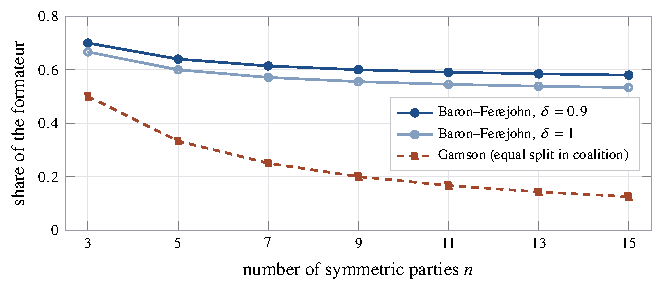
\includegraphics[width=0.62\linewidth]{figures/fig_bf_vs_gamson.pdf}
\caption{The puzzle in the symmetric case: the formateur's equilibrium share under Baron--Ferejohn
(solid) and the equal split prescribed by Gamson's law (dashed), as the number of parties grows.}
\label{fig:bfgamson}
\end{figure}

We study the question computationally. Parties are reinforcement-learning (RL) agents in a configurable
game of government formation that nests the Baron--Ferejohn game exactly and adds, one switch at a time,
the institutional features that have been proposed as explanations of Gamson's law: repeated terms,
exits, the recognition rule, heterogeneous and private valuations of ministries, ministerial policy and a
demand-based bargaining protocol. Agents are rewarded only by their own payoffs, so any proportionality
must emerge; nothing in the reward refers to fairness. We read learned behaviour through two lenses: as
an approximate equilibrium solver, checked against exact equilibria and by best-response
(exploitability) tests, and as a model of adaptive, boundedly rational parties.

\paragraph{Contributions.}
\begin{enumerate}
\item An open environment and learner for coalition bargaining: one permutation-equivariant attention
policy with masked autoregressive proposal heads serves any number of parties and ministries, and is
trained by PPO on each agent's own decision sequence (\cref{sec:model,sec:learning}).
\item Exact benchmarks: the Baron--Ferejohn solution, embedded in the environment, and an exact
backward-induction solver for our demand protocol, whose equilibrium is not covered by published results
(\cref{sec:theory}).
\item A mechanism map of the learned formateur premium in three currencies: number of ministries, the
formateur's own valuation, and policy-setting ministries (\cref{sec:mech}).
\item Pre-registered tests of the bargaining protocol, including a decisive test of whether learned
shares follow seats or voting weights (\cref{sec:protocol}).
\item An out-of-sample confrontation with \RealN{} real coalition cabinets, including the agents' own
cabinets in the same parliaments and a direct test of seats against voting weights in real data
(\cref{sec:real}).
\end{enumerate}

\paragraph{Answer in brief.} Learning parties do not produce seat-proportionality as such. They favour
the formateur exactly as far as the protocol gives it proposal power, and otherwise divide by voting
weight; information and policy motives change the currency of the premium, not its existence. Real
cabinets follow seats even where voting weights disagree.

% =====================================================================
\section{Related work}\label{sec:related}
\paragraph{Gamson's law.} Since \citet{browne1973}, regressions of portfolio shares on within-coalition
seat shares have found slopes near one and very tight fits, also when ministries are weighted by
salience \citep{warwick2001,warwick2006}. Small partners receive slightly more than proportional shares.
\citet{ansolabehere2005} show that a formateur advantage appears when strength is measured by minimal
integer voting weights. Explanations of proportionality include pre-electoral pacts
\citep{carroll2007}, uncertainty and complexity \citep{falco2013}, commitment to a coalition before the
division \citep{kamm2024} and within-party bargaining \citep{cox2021}.

\paragraph{Bargaining theory.} In the closed-rule model \citep{baron1989} the proposer extracts a premium
whose size depends on patience and the number of parties; stationary equilibrium payoffs are unique
\citep{eraslan2002}. With weighted voting, expected payoffs follow voting weights and recognition
probabilities while the realised proposer premium remains \citep{snyder2005}; recognition rules can
support almost any expected division \citep{kalandrakis2006}. Policy can be traded for office
\citep{baron1991,laver1996}. Demand bargaining \citep{morelli1999} predicts no proposer premium and
shares proportional to voting weights for specific move orders; \citet{montero2007} give a
counterexample to the general claim and \citet{montero2011} restore proportionality when parties move in
decreasing order of weight. Our protocol fixes neither order, so we solve it directly.

\paragraph{Learning and experiments.} Laboratory subjects give proposers less than the theory predicts
\citep{frechette2003} and react less to the protocol than theory suggests \citep{frechette2005}.
Learning dynamics can settle on outcomes that are not subgame perfect, because responses that are rarely
tested on the path of play are never corrected \citep{gale1995,fudenberg1993,fudenberg1998}. Deep
multi-agent RL has been used for negotiation \citep{lewis2017}, team formation in weighted voting games
\citep{bachrach2020}, economic policy design \citep{zheng2022} and pricing \citep{calvano2020}. To our knowledge, no prior study combines the three elements used here: learning agents in a
configurable cabinet-bargaining game, validation against protocol-specific exact equilibria including
best-response tests, and confrontation with real cabinet allocations. Our contribution is this
combination, not any single component.

% =====================================================================
\section{Model}\label{sec:model}
\subsection{The cabinet bargaining game}
A parliament has parties $\mathcal N=\{1,\dots,n\}$ with seats $w_i$, total $W$ and quota
$q=\lfloor W/2\rfloor+1$; a coalition $C$ is winning if $w(C)=\sum_{i\in C}w_i\ge q$. There are $m$
ministries with salience $\sigma_k$ and, optionally, party-specific valuations
$\nu_{ik}=(1-\xi)\sigma_k+\xi\,\epsilon_{ik}$ with $\epsilon_{i\cdot}$ drawn from a Dirichlet
distribution. Each period without a cabinet is a formation round (\cref{fig:env}).

\begin{figure}[t]\centering
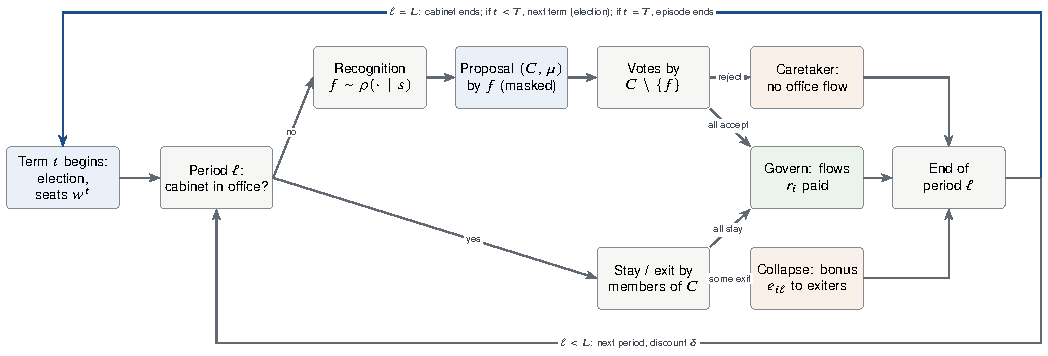
\includegraphics[width=\linewidth]{figures/fig_environment.pdf}
\caption{One period of the environment under the proposal protocol. Without a cabinet, a formateur is
recognised and proposes a coalition and an allocation, which forms the cabinet if every named partner
accepts; otherwise a caretaker period passes. A governing cabinet pays per-period flows; with exits,
members may leave and collapse it.}\label{fig:env}
\end{figure}

\paragraph{Proposal protocol.} A formateur $f$ is drawn from the recognition rule $\rho$ (uniform or
proportional to seats). It proposes a winning coalition $C\ni f$ and an allocation $\mu:\{1..m\}\to C$
(or, with a divisible surplus, shares $p\in\Delta(C)$). The cabinet forms if every partner in $C$
accepts; otherwise the period is lost and the next round is discounted by $\delta$.

\paragraph{Demand protocol.} A first mover is recognised by $\rho$; the others move in a uniformly
random order. Each mover either demands a share of a divisible surplus on a 1\% grid, or \emph{closes}: it
forms a cabinet with the cheapest winning set of earlier demands whose sum is at most one (ties: fewer
members first) and takes the residual. If nobody closes, the round fails. This differs from
\citet{morelli1999}, where the first mover chooses the order of moves.

\paragraph{Payoffs.} A governing member receives $r_i=\sum_{k:\mu(k)=i}\nu_{ik}-\lambda\,\tfrac1d
\sum_h|y_h-z_{ih}|$ per period: the value of its ministries minus a policy loss, where $z_i$ is its
ideal point and, with ministerial policy, the holder of a dimension's lead ministry sets policy $y_h$ on
that dimension. A member that exits receives a random exit bonus. Rewards are individual; there is no
fairness term.

\paragraph{Mechanisms.} Each candidate explanation is a switch: repeated terms with elections (M1),
the demand protocol (M2), private valuations (M4, with heterogeneous values M5), exits (M8), ministerial
policy (M9) and seat-proportional recognition (M10). The \emph{base} game has indivisible ministries and
every mechanism off; E$^\star$ has all of them on. Level E0 is the symmetric Baron--Ferejohn game with a
divisible surplus. The game is a partially observable stochastic game; private valuations and ideal
points are observed only by their owner.

\paragraph{Measurement.} On every installed cabinet $c$ with portfolio-holding members we estimate the
standard regression
\begin{equation}\label{eq:reg}
p_{ic}=\alpha+\beta\,s_{ic}+\gamma\,F_{ic}+\varepsilon_{ic},
\end{equation}
with $p_{ic}$ the share of ministries, $s_{ic}$ the within-coalition seat share and $F_{ic}$ the
formateur dummy (for real cabinets, the prime minister's party). Gamson's law is
$(\alpha,\beta,\gamma)=(0,1,0)$; $\gamma$ is the seat-controlled formateur premium and our headline
statistic. Because the premium may move to other currencies, we estimate~\eqref{eq:reg} also with each
party's share of the value \emph{it} places on ministries (value premium) and its share of policy-setting
ministries (lead premium), and with Banzhaf voting power or minimal integer voting weights in place of
seats.

\subsection{Theoretical benchmarks}\label{sec:theory}
\begin{proposition}[Symmetric Baron--Ferejohn benchmark]\label{prop:bf}
In level E0 with $n$ odd, equal seats, uniform recognition and discount $\delta$, the stationary
subgame-perfect equilibrium in stage-undominated voting strategies has the first proposal accepted; the
formateur offers $\delta/n$ to $(n-1)/2$ partners and keeps $x^{\BF}_f=1-\delta(n-1)/(2n)$.
\end{proposition}
\noindent The environment embeds the Baron--Ferejohn game exactly when a cabinet governs forever and
shares are paid as per-period flows; the proof is in \cref{app:proofs}. For weighted parliaments we
compute stationary equilibria with a homotopy root finder certified by a linear-programming residual
check (\code{cabinet/bf\_solver.py}).

\paragraph{Exact equilibrium of our demand protocol.} Published results do not cover our variant, so we
compute the subgame-perfect equilibrium of the game as implemented, with demands on a finite grid; the
solution is exact for that finite game, not for every demand-bargaining model. We compute it by backward induction over every history of grid demands and
every move order, with failure payoffs $\delta V_i$ iterated to a fixed point in the ex-ante values $V$
(\code{cabinet/demand\_solver.py}, \cref{app:solver}). It agrees with an independently written brute-force solver and with the environment's closing rule
(\cref{app:solver}). The results do not depend on the tie-breaking rule, the grid (1\% and 2\%; 2.5\%
and 4\% for five parties) or patience ($\delta\in\{0.5,0.9,0.95\}$):
\begin{itemize}
\item three equal parties: the first two movers split 0.50/0.50; five equal parties: the first three
movers take about one third each;
\item 45/35/20 seats: \emph{every} pair is winning, and whichever pair forms splits 0.50/0.50, whatever
its seats;
\item 40/30/25/5 seats: the 5-seat party is a dummy (never pivotal) and gets nothing; two of the large
parties split 0.50/0.50.
\end{itemize}
The undercutting logic is simple: under the cheapest-set rule an earlier demand above the closer's
residual is replaced by a cheaper later demand, so demands are competed down to the split of the minimal
winning coalition. The equilibrium is proportional to minimal integer voting weights, here $(1,1,1)$ and
$(1,1,1,0)$, not to seats. Gamson's law predicts 0.56/0.44 to 0.69/0.31 for the 45/35/20 pairs.

% =====================================================================
\section{Learning framework}\label{sec:learning}
\paragraph{Policy.} All parties share one network (\code{cabinet/policy.py}). The observation of a party
is a \emph{set} of party tokens (seat share, recognition probability, roles, current offers, the last
cabinets), a set of ministry tokens (salience, own valuation, policy dimension), pair features and a
context vector (phase, quota, $\delta$, $\lambda$, expected terms). Two attention blocks make the policy
permutation-equivariant, so it applies to any $n$ and $m$ and treats relabelled parties identically.
Proposals are decoded autoregressively with masks that keep every proposal feasible: include or exclude
each party in order of seats, with the quota enforced, then point every ministry to a coalition member;
for a divisible surplus, a 1\% grid offer per partner. Voters, exiting members and demanders have their
own heads; the demand head has 101 demand bins and one \emph{close} action. An optional GRU core carries
memory across decisions.

\paragraph{Training.} PPO \citep{schulman2017} with generalised advantage estimation
\citep{schulman2016} is applied to each agent's own sequence of decisions, a semi-Markov decision process
with interval discounts (\code{cabinet/ppo.py}). Advantages are normalised per decision type, and the
vote and exit heads get five times the entropy bonus so that responders keep learning. Each iteration
collects 8192 decisions; runs last 500--2000 iterations. Variants: MAPPO with a centralised critic that
sees private types \citep{yu2022}, fictitious self-play against a pool of past checkpoints
\citep{heinrich2016}, symmetric PSRO \citep{lanctot2017} and the GRU memory. Hyper-parameters
(\cref{app:hp}) were tuned on E0 only.

\paragraph{Exploitability.} For a frozen profile we train a best response by PPO for one randomly drawn
seat while every other seat plays the profile, from the profile's weights and from scratch, and report
the larger per-period gain over 3000 evaluation episodes. Scripted Gamson and Baron--Ferejohn-heuristic
profiles serve as positive controls. A learned best response bounds exploitability from below, so a small
gain means only that no exploit was found at the budget.

\paragraph{Statistics.} Training seeds are the independent units. Each seed's coefficients come from its
own evaluation cabinets; we report means with 95\% intervals over seeds. Before the final runs finished
we committed a pre-registration (\code{docs/PREREGISTRATION.md}) fixing three confirmatory tests with
Holm correction and four descriptive predictions; everything else is exploratory. For real data we use
country-clustered and wild-cluster bootstraps \citep{cameron2008}.

% =====================================================================
\section{Results}\label{sec:results}
\subsection{Benchmark: learned outcomes match Baron--Ferejohn, learned play does not}\label{sec:bench}
In E0, learned formateur shares follow the closed form of \cref{prop:bf} (\cref{fig:e0}, \cref{tab:e0}):
the mean absolute gap over the nine cells is \EzeroAbsGap{}, the mean signed gap \EzeroGap{}, and
\EzeroCellsOK{}/9 cells are within 0.02; shares fall with patience $\delta$ as theory predicts for
$n\le5$. Between 90\% and 100\% of cabinets are minimal winning, and \EzeroFail{} of rounds fail on average. The largest gap is at
$n=7$, $\delta=0.8$, where the learned share stays at about 0.60 for every $\delta$.

\begin{figure}[t]\centering
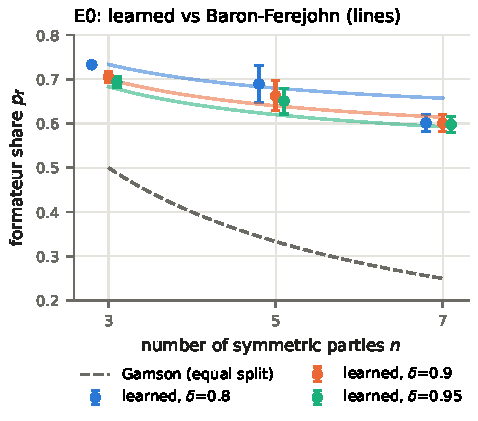
\includegraphics[width=0.62\linewidth]{../figures/fig_e0_benchmark.pdf}
\caption{Benchmark E0: learned formateur share (mean and 95\% CI over 10 seeds) against the closed form
of \cref{prop:bf}; dashed: Gamson's equal split.}\label{fig:e0}
\end{figure}

% generated by scripts/paper_tables.py -- do not edit
\begin{table}[t]\centering\footnotesize
\caption{Benchmark E0 (symmetric closed-rule Baron--Ferejohn game, divisible surplus; 10 seeds, 4000 evaluation episodes each). Gap: learned minus closed-form formateur share, with a 95\% $t$-interval over seeds. Threshold: offer at which a learned voter accepts with probability 1/2. BR gain: payoff a formateur would gain per formation by best-responding to the frozen learned voters (mean over seeds).}\label{tab:e0}
\begin{tabular}{@{}rrcccccc@{}}\toprule
$n$ & $\delta$ & $x^{\mathrm{BF}}_f$ & learned & gap [95\% CI] & threshold & $\delta/n$ & BR gain\\\midrule
3 & 0.8 & 0.733 & 0.733 & \ensuremath{-}0.001 [\ensuremath{-}0.008, +0.007] & 0.205 & 0.267 & 0.013\\
3 & 0.9 & 0.700 & 0.706 & +0.006 [\ensuremath{-}0.008, +0.020] & 0.257 & 0.300 & 0.005\\
3 & 0.95 & 0.683 & 0.694 & +0.010 [\ensuremath{-}0.004, +0.025] & 0.273 & 0.317 & 0.003\\
5 & 0.8 & 0.680 & 0.689 & +0.009 [\ensuremath{-}0.039, +0.057] & 0.079 & 0.160 & 0.056\\
5 & 0.9 & 0.640 & 0.662 & +0.022 [\ensuremath{-}0.017, +0.061] & 0.122 & 0.180 & 0.019\\
5 & 0.95 & 0.620 & 0.650 & +0.030 [\ensuremath{-}0.003, +0.064] & 0.134 & 0.190 & 0.014\\
7 & 0.8 & 0.657 & 0.601 & \ensuremath{-}0.056 [\ensuremath{-}0.079, \ensuremath{-}0.033] & 0.025 & 0.114 & 0.153\\
7 & 0.9 & 0.614 & 0.600 & \ensuremath{-}0.014 [\ensuremath{-}0.036, +0.008] & 0.055 & 0.129 & 0.081\\
7 & 0.95 & 0.593 & 0.598 & +0.005 [\ensuremath{-}0.016, +0.026] & 0.064 & 0.136 & 0.058\\
\midrule
\multicolumn{8}{@{}l}{mean signed gap +0.001; mean absolute gap 0.017; 6/9 cells within 0.02}\\
\bottomrule\end{tabular}\end{table}


Matching outcomes is not equilibrium play. Probing learned voters with synthetic offers shows acceptance
thresholds well below the reservation value $\delta/n$ for $n\ge5$ (\cref{tab:e0}). At the offers
formateurs actually make, the probe agrees with on-path behaviour (acceptance near one, failure near
zero), but against the frozen voters a formateur best response would gain up to \BrGainSeven{} per
formation at $n=7$ and \BrGainFive{} at $n=5$, by offering far less
(\code{scripts/bf\_best\_response.py}). Formateurs never try such offers, so voters are never taught to
reject them: the self-confirming pattern of learning in games \citep{fudenberg1993,gale1995}. As in the
laboratory \citep{frechette2003}, the proposer ends up with less than the theory gives it at large $n$.
A best response trained by PPO against the E0 profile gains \GainEzero{} per period
(\GainEzeroRel{} of a seat's payoff), confirming that the exploitability test detects such gaps.

\subsection{Proposal bargaining: the premium changes currency}\label{sec:mech}
% generated by scripts/paper_tables.py -- do not edit
\begin{table}[t]\centering\footnotesize
\caption{Formateur coefficient $\hat\gamma$ of regression~\eqref{eq:reg} by configuration (mean $\pm$ 95\% half-width over seeds). Counted: share of ministries. Value: share of the value each party places on ministries. Lead: share of policy-setting ministries (only with M9). $\tilde D_G$: floor-adjusted Gamson distance. Configurations with 2--3 seeds are exploratory; the confirmatory tests are in Section~\ref{sec:protocol}.}\label{tab:mech}
\begin{tabular}{@{}lccccc@{}}\toprule
configuration & $\hat\gamma$ counted & $\hat\gamma$ value & $\hat\gamma$ lead & $\tilde D_G$ & seeds\\\midrule
base game (all mechanisms off) & +0.249 $\pm$ 0.038 & -- & -- & 0.132 & 5\\
+ repeated terms (M1) & +0.291 $\pm$ 0.062 & -- & -- & 0.154 & 3\\
+ repeated, patient & +0.320 $\pm$ 0.041 & -- & -- & 0.182 & 3\\
+ heterogeneous public values (M5) & +0.172 $\pm$ 0.147 & +0.131 $\pm$ 0.112 & +0.227 $\pm$ 0.159 & 0.149 & 3\\
+ private values (M4+M5) & \ensuremath{-}0.036 $\pm$ 0.009 & +0.107 $\pm$ 0.010 & \ensuremath{-}0.032 $\pm$ 0.024 & 0.072 & 5\\
+ exits (M8) & +0.223 $\pm$ 0.118 & -- & -- & 0.138 & 3\\
+ ministerial policy (M9) & \ensuremath{-}0.029 $\pm$ 0.019 & \ensuremath{-}0.029 $\pm$ 0.019 & +0.803 $\pm$ 0.061 & 0.089 & 5\\
+ seat recognition (M10) & +0.159 $\pm$ 0.048 & -- & -- & 0.098 & 5\\
\addlinespace
E$^\star$ (all on) & +0.052 $\pm$ 0.034 & +0.205 $\pm$ 0.035 & +0.156 $\pm$ 0.056 & 0.093 & 10\\
E$^\star$ $-$ repeated terms & \ensuremath{-}0.040 $\pm$ 0.062 & +0.105 $\pm$ 0.059 & \ensuremath{-}0.004 $\pm$ 0.062 & 0.098 & 3\\
E$^\star$ $-$ private values & +0.221 $\pm$ 0.040 & +0.200 $\pm$ 0.040 & +0.348 $\pm$ 0.100 & 0.108 & 3\\
E$^\star$ $-$ heterog. values & +0.210 $\pm$ 0.061 & +0.210 $\pm$ 0.061 & +0.203 $\pm$ 0.570 & 0.090 & 3\\
E$^\star$ $-$ exits & +0.207 $\pm$ 0.144 & +0.340 $\pm$ 0.136 & +0.252 $\pm$ 0.155 & 0.097 & 3\\
E$^\star$ $-$ ministerial policy & +0.053 $\pm$ 0.086 & +0.211 $\pm$ 0.082 & +0.040 $\pm$ 0.071 & 0.093 & 3\\
E$^\star$ $-$ seat recognition & +0.092 $\pm$ 0.091 & +0.244 $\pm$ 0.091 & +0.168 $\pm$ 0.103 & 0.116 & 3\\
\addlinespace
E$^\star$, MAPPO & +0.037 $\pm$ 0.029 & +0.188 $\pm$ 0.029 & +0.124 $\pm$ 0.049 & 0.085 & 10\\
E$^\star$, fictitious self-play & +0.065 $\pm$ 0.123 & +0.219 $\pm$ 0.123 & +0.153 $\pm$ 0.241 & 0.094 & 3\\
E$^\star$, GRU memory & +0.040 $\pm$ 0.126 & +0.196 $\pm$ 0.123 & +0.185 $\pm$ 0.260 & 0.097 & 3\\
E$^\star$, memoryless & \ensuremath{-}0.006 $\pm$ 0.041 & +0.142 $\pm$ 0.041 & +0.069 $\pm$ 0.183 & 0.096 & 3\\
E$^\star$, 12 ministries & \ensuremath{-}0.059 $\pm$ 0.129 & +0.147 $\pm$ 0.135 & +0.548 $\pm$ 0.476 & 0.122 & 3\\
\addlinespace
base, 4$\times$ training & +0.295 $\pm$ 0.046 & -- & -- & 0.158 & 2\\
+ private values, 4$\times$ & \ensuremath{-}0.004 $\pm$ 0.005 & +0.139 $\pm$ 0.017 & \ensuremath{-}0.028 $\pm$ 0.262 & 0.070 & 2\\
+ policy, 4$\times$ & +0.007 $\pm$ 0.268 & +0.007 $\pm$ 0.268 & +0.770 $\pm$ 0.983 & 0.085 & 2\\
E$^\star$, 4$\times$ & +0.088 $\pm$ 0.520 & +0.240 $\pm$ 0.517 & +0.158 $\pm$ 0.127 & 0.090 & 2\\
base, PSRO & +0.301 & -- & -- & -- & 1\\
E$^\star$, PSRO & +0.070 & -- & -- & -- & 1\\
\bottomrule\end{tabular}\end{table}


\Cref{tab:mech} and \cref{fig:mech} report the formateur coefficient as mechanisms are added to the base
game or removed from E$^\star$. The base game keeps a substantial premium ($\hat\gamma=\BaseGamma$,
\LongBaseG{} with four times the training budget), and it emerges with training rather than being present
from the start (\cref{fig:curves} in \cref{app:curves}). Repeated terms, even with patient agents and memory, exits, the
recognition rule and heterogeneous public valuations reduce it at most partially. Every learner
(IPPO, MAPPO, fictitious self-play, PSRO, GRU) reproduces the pattern.

\begin{figure}[t]\centering
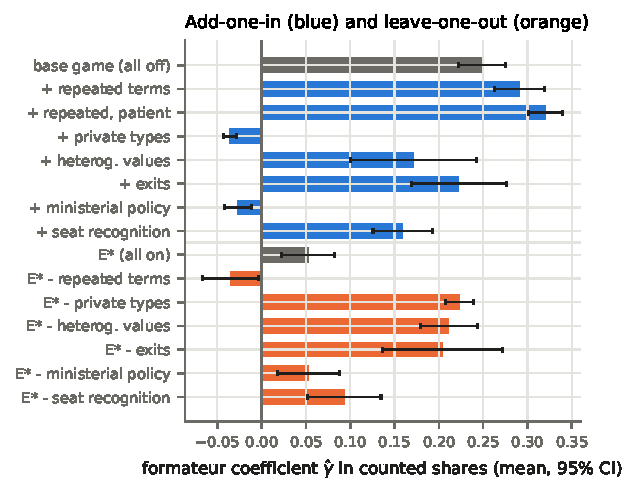
\includegraphics[width=0.7\linewidth]{../figures/fig_mechanisms.pdf}
\caption{Formateur coefficient $\hat\gamma$ in counted shares when a mechanism is added to the base game
(blue) or removed from E$^\star$ (orange); mean and 95\% CI over seeds.}\label{fig:mech}
\end{figure}

Two mechanisms remove the \emph{counted} premium when added alone: private valuations (\MfourGamma) and
ministerial policy (\MnineGamma). In E$^\star$ the counted premium is small (\EstarGamma), and it returns
(0.21--0.22) when private valuations, heterogeneous valuations (without which private types carry no
information) or exits are removed, but not when ministerial policy is removed. But the premium does not vanish.
In each party's share of the value it places on ministries the formateur coefficient is \MfourGnu{}
with private valuations and \EstarGnu{} in E$^\star$, and with ministerial policy the formateur holds the
policy-setting ministries (coefficient \MnineGlead). Both persist with four times the training. The
formateur gives partners more ministries but keeps the ones it values most, or keeps policy control:
the premium changes currency.

\subsection{Demand bargaining follows voting weights}\label{sec:protocol}
On the same random 3--8-party parliaments (\NprotSeeds{} seeds per protocol), demand bargaining lowers
the formateur coefficient by \HoneDiff{} relative to proposal bargaining (95\% CI \HoneLo--\HoneHi; exact
permutation $p=\HoneP$, H1) and raises the seat slope by \HtwoDiff{} (\HtwoLo--\HtwoHi; H2). The demand
coefficient is within $\pm0.05$ of zero (\HthreeMean, 90\% CI \HthreeLo{} to \HthreeHi; H3). All three
pre-registered tests pass after Holm correction. The small negative value is an exploration artefact: the
single close action competes with 101 demand bins, and with five times the entropy on the demand head the
coefficient becomes \ExpDemG{} (seat slope \ExpDemB).

\begin{table}[t]\centering\footnotesize
\caption{Who gets what in fixed parliaments (divisible surplus, $\delta=0.9$, seat-proportional
recognition; learned: \AfDemSeeds{} seeds per protocol, every coalition that forms).}\label{tab:fixed}
\begin{tabular}{@{}lll@{}}\toprule
 & 45/35/20 (each pair) & 40/30/25/5 \\\midrule
Gamson's law (seats) & larger party 0.56--0.69 & dummy gets $5/w(C)$ if included\\
demand: exact equilibrium & 0.50/0.50 & 0.50/0.50, dummy never included\\
demand: learned & $0.50\pm\AfDemMaxDev$ (seat slope \AfDemSlope) & $0.50\pm\AtDemMaxDev$, dummy included \AtDemDummy\\
proposal: weighted BF & formateur $\approx0.70$ & formateur $\approx0.71$\\
proposal: learned & formateur \AfPropFormLo--\AfPropFormHi & formateur \AtPropFormLo--\AtPropFormHi\\
\bottomrule\end{tabular}\end{table}

Is this Gamson's law? The fixed parliaments of \cref{tab:fixed} separate seats from voting weights.
Learned demand agents reproduce the exact equilibrium of \cref{sec:theory}: every 45/35/20 pair splits within \AfDemMaxDev{} of 50/50 (pre-registered prediction P1: every seed's
slope below 0.5; seat slope \AfDemSlope, seed-level 95\% CI \PoneLo{} to \PoneHi{}, which excludes
Gamson's slope of 1), and the
dummy party in 40/30/25/5 is never included (P2). Learned proposal agents give the formateur
\AfPropFormLo--\AfPropFormHi, close to the weighted Baron--Ferejohn solution (P3). Learned demand shares
thus follow voting weights; the seat slope of 0.8 in random parliaments arises because seats and voting
weights are correlated there. In symmetric demand games with default exploration the closer is
under-paid (\LockinCloserThree{} with three parties, \LockinCloserFive{} with five) and a best response
gains \GainDemand{} per period; with more exploration of demands the closer gets \ExploreCloserThree{}
and \ExploreCloserFive{}, moving to the equilibrium values 0.50 and about 0.34, and the best-response gain
falls to 0.029.

\subsection{Real cabinets}\label{sec:real}
We use ministers per party from the Seki--Williams party government data \citep{seki2014}, linked to
ParlGov parliaments \citep{parlgov}: \RealN{} majority coalition cabinets in 31 countries, 1988--2014,
with the prime minister's party as the formateur. Real cabinets were never used for training or tuning.
\emph{Samples.} All regressions and robustness checks use the \RealN{} cabinets. Split predictions use
\RealNcommon{}: the agents' parliaments contain the eight largest parties, which excludes the 12 cabinets
with a member outside them. The key-ministry test uses the \KeyN{} cabinets (25 countries) that can be
matched to the Seki--Williams minister records with at least four partisan senior ministers, a prime
minister's party identifiable among them, a partner holding a ministry, and at least one key ministry.
The equal-weight test uses the \WvsPairs{} partner pairs with equal minimal integer weight and seat shares
differing by more than 0.02. Coalition choice uses ParlGov's 242 Western European parliaments.

\begin{table}[t]\centering\small
\caption{Real cabinets: the prime-minister coefficient $\hat\gamma$ of~\eqref{eq:reg} under different
specifications, with wild-cluster bootstrap 95\% CIs (31 countries). Bottom: partners with equal minimal
integer voting weight but different seats (\code{scripts/real\_weights\_vs\_seats.py}).}\label{tab:realrob}
\begin{tabular}{@{}lccc@{}}\toprule
specification & $\hat\gamma$ & 95\% CI & $R^2$\\\midrule
seat shares & \RobBaseG & \RobBaseLo{} to \RobBaseHi & \RobBaseRtwo\\
seat shares, intercept $\alpha/k$ (cabinet size) & \RobOverkG & \RobOverkLo{} to \RobOverkHi & \RobOverkRtwo\\
seat shares + largest-party dummy & \RobLargestG & \RobLargestLo{} to \RobLargestHi & \RobLargestRtwo\\
minimal integer voting weights & \RobWeightsG & \RobWeightsLo{} to \RobWeightsHi & \RobWeightsRtwo\\
seats and weights together & \RobBothG & \RobBothLo{} to \RobBothHi & \RobBothRtwo\\\midrule
\multicolumn{4}{@{}p{0.9\linewidth}@{}}{equal voting weight, different seats: seat slope \WvsSlope{}
(95\% CI \WvsLo--\WvsHi), \WvsPairs{} pairs; without the PM's party \WvsNoPm{} (\WvsNoPmN{} pairs)}\\
\bottomrule\end{tabular}\end{table}

\paragraph{The real regression.} Real cabinets follow Gamson's law closely: share $=\RealA+\RealB\,s+
\RealG\,F$, $R^2=\RealRtwo$; leaving out any one country keeps $\hat\gamma$ between \LocoLo{} and
\LocoHi. The formateur premium depends on the measure of strength (\cref{tab:realrob}): none relative to
seats, \RobWeightsG{} relative to minimal integer voting weights, as \citet{ansolabehere2005} report, and
\RobLargestG{} with a largest-party control (identified by the \RobPmNotLargest{} cabinets whose prime
minister does not come from the largest partner). Seats fit better than weights and absorb the weight
effect when both enter. The most direct comparison is between partners with \emph{equal} voting weight but different seats,
where demand theory and our learned demand agents predict equal shares and Gamson's law predicts
seat-proportional ones. Regressing each pair's difference in portfolio shares on its difference in seat
shares, through the origin and with a prime-minister indicator, gives a seat slope of \WvsSlope{}; the
95\% interval \WvsLo--\WvsHi{} comes from a bootstrap over countries, because pairs from the same
cabinet or country are not independent. The estimate supports seat-based division but is imprecise, and
it is weaker when the prime minister's party is not involved (\WvsNoPm, \WvsNoPmN{} pairs).

\paragraph{Key ministries.} If the real premium were hidden in quality, as with our agents, prime
ministers' parties should hold more than their share of the key ministries. On \KeyN{} cabinets they hold
\KeyShare{} of finance, foreign affairs, interior, defence and justice, against \KeyCount{} of all
ministers (difference \KeyDiff, 95\% CI \KeyDiffLo{} to \KeyDiffHi): no detectable premium, in line with
salience-weighted evidence \citep{warwick2006}.

\begin{figure}[t]\centering
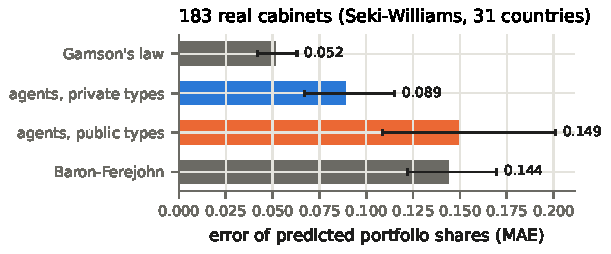
\includegraphics[width=0.62\linewidth]{../figures/fig_real.pdf}
\caption{Predicting the portfolio split of real coalition cabinets given the real coalition and prime
minister: mean absolute error per party with country-clustered 95\% CIs.}\label{fig:real}
\end{figure}

\paragraph{Prediction.} Given each real coalition and prime minister, policies trained only on random
parliaments predict the split with mean absolute error \MaePrivLo--\MaePrivHi{} per party when they have
private valuations, and \MaePubLo--\MaePubHi{} with public valuations; Baron--Ferejohn errs by \MaeBF{}
and Gamson's law by \MaeGamson{}, the best in every leave-one-country-out sample (\cref{fig:real}).

\begin{table}[t]\centering\small
\caption{Regression~\eqref{eq:reg} with seat shares and with Banzhaf voting power ($\hat\gamma_{bz}$) on
real cabinets and on the cabinets that agents form themselves in the same \RealN{} parliaments (ranges over
seeds: 10 per protocol, 3 otherwise).}\label{tab:own}
\begin{tabular}{@{}lcccc@{}}\toprule
 & $\hat\beta$ & $\hat\gamma$ & $\hat\gamma_{bz}$ & $R^2$\\\midrule
real cabinets & \RealB & \RealG & \RealGbz & \RealRtwo\\
demand protocol & \OwnDemB & \OwnDemG & \OwnDemGbz & \OwnDemRtwo\\
\quad with more exploration & \OwnExpB & \OwnExpG & \OwnExpGbz & \OwnExpRtwo\\
proposal protocol & \OwnPropB & \OwnPropG & \OwnPropGbz & \OwnPropRtwo\\
E$^\star$ (proposal, all mechanisms) & \OwnWideB & \OwnWideG & \OwnWideGbz & \OwnWideRtwo\\
\bottomrule\end{tabular}\end{table}

\paragraph{Agents in real parliaments.} Left to bargain freely in the real parliaments (\cref{tab:own}),
demand agents with more exploration reproduce the real seat regression almost exactly, although their
rule is voting weight: in most real parliaments the two are close. E$^\star$ agents match the small
premium relative to voting power; proposal agents overshoot it. Restricting the agents' cabinets to those
that reproduce the real coalition barely changes the demand slope (\OwnDemMatchB), so coalition
selection is not what makes it seat-like. Choosing coalitions in 242 Western European parliaments, the
agents pick the governing coalition in \PgLearned{} of cases, similar to Riker's minimal-seat rule
(\PgRiker) and below an ideologically connected rule (\PgIdeology).

\subsection{Reliability}\label{sec:reliability}
% generated by scripts/paper_tables.py -- do not edit
\begin{table}[t]\centering\footnotesize
\caption{Estimated exploitability: per-period gain of a best response trained by PPO for one random seat against the frozen profile (larger of a warm and a from-scratch start), also relative to the profile seat's payoff. Scripted positive controls (proposal protocol only) have no network weights to start from, so their best response is trained from scratch only; with a weak budget its gain can be slightly negative.}\label{tab:exploit}
\begin{tabular}{@{}lrcccc@{}}\toprule
profile & BR iters & gain & relative & Gamson ctrl. & BF-heur. ctrl.\\\midrule
E$^\star$ (IPPO) & 400 & 0.015 & 10\% & 0.037 & 0.088\\
E$^\star$ (MAPPO) & 150 & 0.018 & 12\% & 0.023 & 0.094\\
E$^\star$ (IPPO, 3 seeds) & 150 & 0.016 & 10\% & 0.020 & 0.076\\
base game (3 seeds) & 150 & 0.017 & 7\% & 0.008 & \ensuremath{-}0.004\\
E0 (BF benchmark) & 300 & 0.040 & 20\% & 0.019 & 0.037\\
random parliaments, proposal & 400 & 0.033 & 18\% & -- & --\\
random parliaments, demand & 400 & 0.034 & 19\% & -- & --\\
symmetric demand, default exploration & 300 & 0.143 & 57\% & -- & --\\
symmetric demand, more exploration & 300 & 0.029 & 12\% & -- & --\\
\bottomrule\end{tabular}\end{table}


\Cref{tab:exploit} reports estimated exploitability. Best responses gain \GainLong{} per period against
E$^\star$ (\GainLongRel{} of a seat's payoff) and about a fifth of a seat's payoff against agents on random
parliaments under either protocol, against \GainLongGamson{} and \GainLongMyopic{} for scripted Gamson and
Baron--Ferejohn-heuristic profiles. The test has power at 300--400 iterations (it finds the gaps of
\cref{sec:bench}), but at 150 iterations its controls in the base game were not detected, so budgets
matter. Cross-play between independently trained runs costs \CmSame{} per period within an algorithm and
\CmAcross{} across algorithms: independent runs settle on compatible conventions. Learned profiles are
approximate equilibria, and our conclusions are about the allocation rules they settle on, which are
stable across seeds, learners and training budgets.

% =====================================================================
\section{Discussion}\label{sec:discussion}
\paragraph{Answer to the question.} Should cabinets allocate proportionally or favour formateurs? Read
positively, as a question about what self-interested bargaining produces, our answer is: neither rule
emerges unconditionally. Learning parties favour the formateur exactly as far as the rules give it
proposal power (\cref{sec:mech}); when parties bargain by demands, the premium disappears but shares
follow voting weights (\cref{sec:protocol}). Private information and policy motives do not remove the
proposer's advantage; they move it into the ministries the formateur values or into policy control, which
counting ministries cannot see. Real cabinets, in contrast, divide by seats even where voting weights
disagree, show at most a small premium relative to voting weights, and no detectable premium in key
ministries (\cref{sec:real}).

\paragraph{Implications.} Gamson's law is therefore not the equilibrium of either canonical bargaining
protocol, as learned by self-interested agents. Demand bargaining comes closest, and in real parliaments,
where seats and voting weights are correlated, its learned allocations reproduce the real regression.
Where seats and weights diverge, the available evidence has real cabinets siding with seats. This points to mechanisms outside these
bargaining models: commitments to a coalition before the division \citep{kamm2024}, pre-electoral pacts
\citep{carroll2007}, intra-party bargaining \citep{cox2021} or a proportionality norm. For the
learning literature, the benchmark shows how outcome-level validation can hide non-equilibrium play: the
learned profile matches Baron--Ferejohn shares while leaving a profitable deviation untried.

\paragraph{Limitations.} Sizes are scaled down ($n\le5$ in the mechanism experiments, 3--8 in random and
real parliaments, $m=6$). Learned profiles are approximate equilibria, and exploitability estimates are
lower bounds. The prime minister's party is a proxy for the formateur. Real shares count ministers;
salience enters only through the key-ministry test, and the test of the currency shift in real data with
party-specific manifesto salience was not run. The demand head offers one close action against 101 demand
bins, which slows learning to close; the exploration runs show that our conclusions do not depend on it.
The normative comparison of allocation conventions (delay, durability, welfare) was outside the scope of
the experiments reported here.

% =====================================================================
\section{Conclusion}\label{sec:conclusion}
Modelling parties as learning agents bargaining over cabinets shows that the formateur premium is a
property of proposal power, not of strategic bargaining as such, and that its absence under demand
bargaining yields division by voting weight, not by seats. Information and policy motives change where the
premium appears rather than whether it exists. Where seats and voting weights disagree, real cabinets follow seats, unlike any protocol we trained, so
the explanation of Gamson's law must include rules or norms beyond the canonical bargaining models.

\paragraph{Reproducibility.} Code, configurations, trained agents, raw results, the pre-registration and a
map from every claim to its result file and script are at \url{\repo}
(\code{docs/RESULTS\_AUDIT.md}). Every number in this paper is generated from the result files
(\code{scripts/make\_figures.py}, \code{scripts/paper\_tables.py}); 32 automated tests tie the code to the theory (\code{tests/test\_core.py}). We re-ran every analysis
and the test suite from a fresh clone of the repository; all outputs were identical to the committed
ones.

\bibliographystyle{plainnat}
\bibliography{references}

% =====================================================================
\appendix
\section{Proof of Proposition~\ref{prop:bf}}\label{app:proofs}
\begin{proof}[Embedding]
Fix a stationary profile at the divisible level with a cabinet that governs forever, no exits and
constant $\rho$. A member $j$ of an accepted cabinet with share $p_j$ receives $p_j/(1-\delta)$; after a
rejection it gets nothing this period and $\delta V_j$ afterwards, with $V_j=v_j/(1-\delta)$.
Stage-undominated voting accepts if and only if $p_j\ge\delta v_j$. A proposal passes only if $C\ni f$,
$w(C)\ge q$ and every partner receives at least $\delta v_j$, so the best passing proposal pays exactly
$\delta v_j$ to a cost-minimising coalition and leaves $x_f=1-\delta c_f(v)$, where $c_f(v)$ is the
minimal $\sum_{j\in S}v_j$ over sets $S$ with $w(S\cup\{f\})\ge q$. Because the grand coalition is
winning, $c_f(v)\le1-v_f$ and $x_f\ge1-\delta+\delta v_f>\delta v_f$, so passing is optimal. These are
exactly the conditions of the closed-rule game of \citet{baron1989}, so stationary strategies and
per-period shares coincide.
\end{proof}
\begin{proof}[Symmetric case]
Conjecture $v_i=1/n$. Voters accept offers of at least $\delta/n$. Every coalition of $f$ and $(n-1)/2$
others costs $(n-1)/(2n)$, so $f$ keeps $x^{\BF}_f=1-\delta(n-1)/(2n)$ and, choosing uniformly among
cheapest coalitions, includes each other party with probability $1/2$. Then
\[
v_i=\tfrac1n\Bigl(1-\tfrac{\delta(n-1)}{2n}\Bigr)+\tfrac{n-1}{n}\cdot\tfrac12\cdot\tfrac{\delta}{n}=\tfrac1n,
\]
confirming the conjecture. By the one-shot deviation principle the profile is a stationary equilibrium;
stationary equilibrium payoffs are unique for quota rules \citep{eraslan2002}.
\end{proof}

\section{The demand-protocol solver}\label{app:solver}
For a move order $\pi$ and a demand grid $G$, let $h=(d_1,\dots,d_k)$ be the demands of the first $k$
movers. The mover at position $k$ can close if some set $S$ of earlier movers satisfies
$w(S)+w_{\pi_k}\ge q$ and $\sum_{j\in S}d_j\le1$; the environment then takes the cheapest such $S$ (ties:
fewer members, then a fixed subset order) and pays the closer $1-\sum_{j\in S}d_j$. Otherwise, or by
choice, it demands $a\in G$ and play moves to $(h,a)$; at the last position a demand ends the round with
payoffs $\delta V$. Backward induction over all $|G|^k$ histories, vectorised over histories, gives every
mover's optimal action; the ex-ante values $V$ are averaged over recognition and random orders and
iterated to a fixed point. Indifferent movers break ties by a fixed rule (close first; then the highest
or the lowest demand), and the reported equilibria are identical under both rules. \paragraph{Verification} (\code{scripts/demand\_solver\_check.py}). (i)~An independent implementation,
a plain recursive backward induction over one history at a time with its own cheapest-set routine, gives
the same ex-ante values and the same on-path outcome for every move order in \SolverCompared{}
configurations (three and five equal parties, 45/35/20, 40/30/25/5; grids of 10\% and 5\%, 10\% only for five parties; both tie
rules), up to single-precision rounding ($10^{-8}$). (ii)~That cheapest-set routine selects the same
coalition as the environment in all \SolverEnvN{} random demand histories with 3--6 parties
(\SolverEnvBad{} mismatches). (iii)~The fixed-point iteration in $V$ stops with residual zero to machine
precision after one or two iterations: on the equilibrium path no round fails, so $\delta V$ only bounds
off-path options and never binds. (iv)~The on-path splits are identical under both tie rules, every grid
and $\delta\in\{0.5,0.9,0.95\}$. Automated tests cover the three-party and dummy-party cases and the
agreement with the brute-force solver (\code{tests/test\_core.py}).

\section{Hyper-parameters}\label{app:hp}
\begin{table}[h]\centering\footnotesize
\caption{PPO hyper-parameters (\code{cabinet/ppo.py}, \texttt{DEFAULT\_HP}), tuned on E0 only.}
\begin{tabular}{@{}ll@{\qquad}ll@{}}\toprule
learning rate & $3\cdot10^{-4}$ (Adam) & decisions per iteration & 8192 (64 environments)\\
GAE $\lambda$ & 0.95 & PPO epochs, minibatches & 4, 4\\
clip & 0.2 & value-loss weight & 0.5\\
entropy bonus & $2\cdot10^{-2}\to2\cdot10^{-3}$ & entropy multiplier, vote/exit & 5\\
embedding width & 64, 4 heads, 2 blocks & demand-entropy multiplier & 1 (5 with more exploration)\\
\bottomrule\end{tabular}\end{table}

\section{Learning curves}\label{app:curves}
\begin{figure}[h]\centering
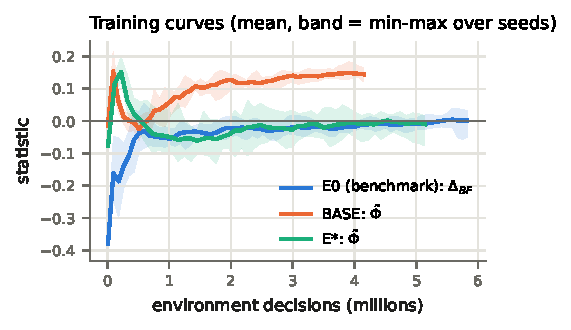
\includegraphics[width=0.8\linewidth]{../figures/fig_curves.pdf}
\caption{Training curves (mean over seeds; band: minimum to maximum). E0: gap of the learned formateur
share to the closed form. Base game and E$^\star$: floor-adjusted formateur premium $\tilde\Phi=
\E[p_f-p_f^{\min}]$, where $p^{\min}$ is the most proportional feasible allocation of the same cabinet.
The premium of the base game is absent early in training and grows with it.}\label{fig:curves}
\end{figure}

\end{document}
